\documentclass[article,a4paper]{article}

\usepackage[utf8]{inputenc}
\usepackage[T1]{fontenc}
\usepackage{changepage}
\usepackage{ragged2e, lipsum}
\usepackage{tabularx, caption, booktabs}
\usepackage{a4wide}
\usepackage{amsmath}
\usepackage{fancyhdr}
\usepackage{adjustbox}
\usepackage[colorlinks=true,linkcolor=black,urlcolor=blue,bookmarksopen=true]{hyperref}
\usepackage{soul}
\usepackage[spanish]{babel}
\usepackage[utf8]{inputenc}
\usepackage[T1]{fontenc}
\usepackage{graphicx}
\usepackage{float}
\usepackage{minted}

\pagestyle{fancy}
\fancyhf{}
\fancyhead[L]{TP1 - 1c2018}
\fancyhead[R]{Teoría de Algoritmos I - FIUBA}
\renewcommand{\headrulewidth}{0.4pt}
\fancyfoot[C]{\thepage}
\renewcommand{\footrulewidth}{0.4pt}
\setlength{\footskip}{17pt}

\begin{document}

\begin{titlepage}
	\hfill
\includegraphics[width=6cm]{fiuba.jpg}
    \centering
    \vfill
    \Huge \textbf{Trabajo Práctico 1}
    \vskip2cm
    \Large [75.29/95.06] Teoría de Algoritmos I\\
    Primer cuatrimestre de 2018
    \vfill
    \begin{flushleft}
    Grupo MinMax
    \end{flushleft}
    \begin{tabular}{|l|c|r|}
	\hline
	Alumno & Padrón & Mail\\
	\hline
	\hline
	del Mazo, Federico & 100029 & delmazofederico@gmail.com\\
	\hline
    Djeordjian, Esteban Pedro & 100701 & edjeordjian@gmail.com\\	
	\hline
	Kristal, Juan Ignacio & 99779 & kristaljuanignacio@gmail.com\\
	\hline
    Raveszani, Nicole & 101031 & nraveszani@gmail.com\\
	\hline
	\end{tabular}
    \vfill
    \vfill
\end{titlepage}

\pagenumbering{gobble}
\tableofcontents
\newpage
\pagenumbering{arabic}
\setcounter{page}{1}

\section{Cálculo Empírico de Tiempos de Ejecución}
\subsection{Complejidad Teórica}
\subsubsection{Selección}

El ordenamiento de selección es uno de los algoritmos de ordenamiento más faciles de implementar. En cada iteracion, se halla el mínimo elemento de la sección del arreglo desordenado y se intercambian las posiciones de este valor y el último elemento. Se reduce en una unidad la sección del arreglo desordenado y al resto se lo considera ordenado.

De acuerdo a nuestra implementación\footnote{Las complejidades de los métodos nativos de las listas de Python 3 fueron sacadas de: \url{https://wiki.python.org/moin/TimeComplexity}} del ordenamiento de selección, la complejidad teórica es:

$\mbox{T seleccion(n)} = \mathcal O(2 + 1 + n * (1 + 1 + 1 + n * (1 + 1) + 1 + 2)) = \mathcal O(n^2 + 6n + n) \in \mathcal O(n^2)$\\

Esto viene de analizar linea por linea teniendo en cuenta:
\begin{itemize}
\item Hacer una asignación y comparar variables: $O(1)$
\item Operadores aritméticos básicos: $O(1)$
\item Sacar la longitud de un arreglo: $O(1)$
\item Hacer un ciclo definido que itera por todo el arreglo: $O(n * f(n))$ siendo $f(n)$ lo que hay dentro del ciclo.
\item Hallar el indice de un elemento: $O(n)$
\end{itemize}

Este ordenamiento itera siempre por el arreglo sin importar su disposicion inicial. Por lo tanto, su peor caso y su caso promedio son iguales al tiempo analizado:

$\mbox{Peor T selecccion(n)} \in O(n^2 + 6n + n) \in O(n^2)$ 

$\mbox{Promedio T selecccion(n)}  \in O(n^2 + 6n + n) \in O(n^2)$


\subsubsection{Inserción}

Inicialmente, se tiene un solo elemento y se lo considera un conjunto ordenado. En cada iteración, se compara al siguiente elemento del conjunto ordenado con su predecesor y se intercambia en caso de ser menor a este. Se itera de esta forma hasta que la condicion anterior no se cumpla. Al igual que el de seleccion, el algoritmo consiste de dos ciclos anidados que recorren el arreglo entero, por lo tanto, el tiempo esperado sera cuadrático.

Este ordenamiento usa las mismas herramientas del ordenamiento de selección. Por lo tanto, con las consideraciones anteriores tomadas, queda:

$\mbox{T seleccion(n)} = \mathcal O( 2 + 1 + n * (2 + 1 + 2 + 2 + 1 + n * (1 + 3)) = \mathcal O(4n^2 + 8n + 3) \in \mathcal O(n^2)$

Siendo la condición de corte que en la iteración el elemento actual no sea menor a lo iterado descendentemente, el peor caso del algoritmo es donde el arreglo inicial esta dispuesto de manera descendente, de tal forma que el ciclo sea ejecutado sin cortes.

$\mbox{Peor T inserción(n)} \in \mathcal O(4n^2 + 8n + 3) \in \mathcal O(n^2)$

Como es claro que encontrar en un arreglo un intervalo ordenado (suficientemente grande) es mucho menos probable que no hacerlo (es decir, para un arreglo de n elementos, de las $n!$ posibles distribuciones de los elementos, solo una estara ordenada, y con un n no demasiado grande, se cumple que $n!-1 \approx n$). Luego, en el caso promedio se tiene que el algoritmo tambien tiene orden cuadratico.

$\mbox{Promedio T inserción(n)} \in \mathcal O(4n^2 + 8n + 3) \in \mathcal O(n^2)$

\subsubsection{Mergesort}

El algoritmo de mergesort es un ordenamiento que utiliza la técnica de División y Conquista, y por lo tanto, para calcular su complejidad teórica va a ser utilizado el Teorema Maestro. Si el arreglo sólo tiene un elemento o ninguno se considera ordenado. En otro caso, el arreglo se subdivide por la mitad creando dos nuevos arreglos. Cada uno de estos arreglos se vuelve a subdividir de forma recursiva hasta que queda un elemento o dos en cada subarreglo. A partir de aqui, cada mitad creada se une de forma ordenada en un nuevo arreglo hasta que queda un único arreglo ordenado.

En cuanto a código se introducen nuevos metodos:

\begin{itemize}
\item \texttt{Append} y \texttt{pop}: $\mathcal O(1)$
\item \texttt{Extend}: $\mathcal O(k)$ siendo k la cantidad de elementos agregados 
\end{itemize}

También es de notar que este es el primer algoritmo donde usamos llamadas recursivas, por su naturaleza de división y conquista.\\

Aplicando el Teorema Maestro: $\mbox{T mergesort(n)} = a * \mbox{T mergesort}(\frac{n}{b}) + f(n^c)$

La cantidad de llamadas recursivas (a) son dos. Cada llamada recursiva divide la entrada inicial a la mitad (b=2). Por último, el tiempo de las llamadas no recursivas es 

$\mathcal O(2 + 2 + 1 + 1 + (n-1) 3 + 1 + 1) = \mathcal O(3n + 5)) \in \mathcal O(n)$\\

Asumiendo un n lo suficientemente grande como para que se requieran intercalar aproximadamente n elementos la mayoría de las veces, por lo que c=1. Se tiene entonces:

$\mbox{T mergesort(n)} = 2 * \mbox{T mergesort} (\frac{n}{2}) + f(n)$

Como $(a = b^c)$, se tiene que: $\mbox{T mergesort(n)} \in \mathcal O(n \log n)$

\hl{Texto sobre peor y promedio caso mergesort}

$\mbox{PeorTmergesort(n)} \in O(n \log n))$

$\mbox{PromedioTmergesort(n)} \mathcal O(2 + 2 + 1 + 1 + (\frac n 2) 3 + \frac n 2 + 1) = \mathcal O(3n + 5)) \in \mathcal O(n \log n)$ \\

\subsubsection{Quicksort}

Al igual que mergesort, quicksort utiliza la tecnica de División y Conquista. Se elige un elemento del arreglo como pivote (en nuestra implementacion se elige al primero) y a partir del pivote se arman tres arreglos: la de todos los elementos menores al pivote, la conformada solo por el pivote y la de todos los elementos mayores al pivote. Con esto se obtiene un orden relativo al pivote. El mecanismo antes descripto se repite recursivamente para cada parte. El arreglo final se obtiene concatenando las sublistas ordenadas. Al igual que en Mergesort, siendo División y Conquista la técnica utlilizada, se usa el Teorema Maestro para calcular su complejidad.

Considerando las complejidades analizadas hasta ahora (en código no hay nada nuevo) y aplicando el Teorema Maestro se tiene:

$Tquicksort(n) = a.Tquicksort(\frac{n}{b}) + f(n^c)$

La cantidad de llamadas recursivas (a) son 2. Para analizar b, se debe considerar dos casos. Por un lado, en el caso promedio, b será igual a 2, ya que en un arreglo arbitrariamente grande, es mucho más probable tomar en cualquier posición a un elemento alejado de las cotas superiores e inferiores que muy próximo a ellas, por lo que la recursión dividirá el problema en “dos partes iguales” (probablemente nunca sean exactamente iguales, pero con un n arbitrariamente grande, las diferencias que puedan existir son despreciables en tanto el pivote elegido no esté lo suficientemente próximo a una cota superior o inferior). El tiempo de las llamadas no recursivas es $O(4n + 4)$, por lo que $c=1$

Para este caso, como $(a = b^c)$ ($2 = 2^1$), se tiene que:

$PromedioTquicksort(n) \in O(n \log n))$

Pero existe un peor caso en donde el pivote elegido es una el menor o el mayor elemento del arreglo, dividiendo el arreglo en dos partes de $1$ y $n-1$ elementos respectivamente. Por lo tanto, usamos como peor caso un arreglo ordenado descendientemente y tomando de pivote el primer elemento del arreglo. Para este peor caso se tiene que b=1, ya los elementos quedan “a la derecha o a la izquierda” del pivote. Para este caso, donde no se puede aplicar el teorema del maestro (porque no hay división y conquista propiamente dicha) queda:

$PeorTquicksort(n) = O( n(4n + 4) ) =  O( 4n^2 + 4n) \in O(n^2)$

\subsubsection{Heapsort}

En el heapsort se utiliza la estructura de cola de prioridad (heap). Se construye un heap de minimos con los elementos del arreglo. Al ser la raiz el menor elemento, se extrae la raiz y se la guarda en la primera posicion del arreglo. De esta forma, se extrae en sucesivas iteraciones la raiz y el elemento es guardado en la siguiente posicion hasta vaciar el heap.

Los tiempos del heap de minimos implementado son:

\begin{itemize}
\item \texttt{Heapify}: $O(x)$
\item \texttt{Upheap}: $O(x)$
\item \texttt{Downheap}: $O(x)$
\item \texttt{Heappop}: $O(x)$
\item \texttt{Heapush}: $O(x)$
\end{itemize}

Considerando todo esto queda: 

$O( n + n +1 + 1 +1+n(1 + \log n  ) = O(3n + 3 + n \log n ) \in O(n \log n)$ 

\hl{Texto sobre peor tiempo y tiempo promedio de heapsort}

$PeorTheapsort(n)  \in O(3n + 3 + n \log n) \in O(n \log n)$

$PromedioTheapsort(n) \in O(3n + 3 +n \log n) \in O(n \log n)$ 

\subsection{Comparación}

\subsubsection{Peores tiempos}

En orden ascendiente de eficiencia:\\

$PeorTinsercion(n) \in O(4n^2 + 9n + 2) \in O(n^2)$

$PeorTselecccion(n) \in O(3n^2 + 8n + 3) \in O(n^2)$ 

$PeorTquicksort(n) \in O(4n^2 + 4n) \in O(n^2)$

$PeorTheapsort(n)  \in O(3n + 3 +n \log n) \in O(n \log n)$

$PeorTmergesort(n) \in O(n \log n)) \in O(n \log n)$

\subsubsection{Tiempos promedio}

En orden ascendiente de eficiencia:\\

$PromedioTinsercion(n) \in O(4n^2 + 9n + 2) \in O(n^2)$

$PromedioTselecccion(n)  \in O(3n^2 + 8n + 3) \in O(n^2)$

$PromedioTheapsort(n) \in O(3n + 3 +n \log n) \in O(n \log n)$ 

$PromedioTmergesort(n) \in O(n \log n)) \in O(n \log n)$

$PromedioTquicksort(n) \in O(n \log n)) \in O(n \log n)$\\

Para poder terminar de ubicar en la escala a quicksort y mergesort, se pone el foco en la complejidad de su parte no recursiva: por parte de quicksort es $O(4n + 4)$, y en el caso de mergesort es $O( \frac{9n}{2} +11 )$. Es decir, la diferencia fundamental en ambos casos es que en el peor caso quicksort será mucho menos eficiente.

\subsection{Peores sets}

\subsubsection{Selección}

Como se ve en el análisis, el comportamiento de este algoritmo no depende de las características del arreglo. En términos más específicos, el algoritmo de selección no es un algoritmo “adaptativo”: su conducta no se ve afectada por ninguna característica del array, por lo cual realizará el mismo número de comparaciones e intercambios entre elementos tanto en el peor caso, en el caso promedio y en el mejor caso (considerando una longitud de arreglo arbitrariamente grande). Sin embargo, un arreglo considerado como el peor valor de entrada posible es un arreglo ordenado de forma descendente, debido a que nuestra implementación se busca el mínimo en cada iteración. Si bien asintóticamente no hay diferencia, diferirá en un valor constante el cual será mayor para un arreglo ordenado de esta forma.

\subsubsection{Inserción}

Este algoritmo sí presenta un peor caso: cuando el arreglo de entrada se encuentra ordenado de forma descendente (y no al revés, según la implementación dada). El bucle interno del algoritmo deberá comparar cada elemento hasta llegar a la primera posición del conjunto, con lo cual realizará el máximo número de comparaciones posibles entre elementos. Esto también está contemplado dentro de su comportamiento en promedio: se destaca el caso en que, si el arreglo estuviera ordenado al revés, el algoritmo terminaría en un orden de O(n) (siendo para este caso trivial, mejor que cualquier ordenamiento).

\subsubsection{Mergesort}

\hl{Como se analizo con el Teorema Maestro, Mergesort es de orden $O(n \log n)$, por lo que no presenta un peor caso para ningun set en general.}

\subsubsection{Quicksort}

Quicksort presenta un caso en que su comportamiento resulta cuadrático: cuando todos (o casi todos) los elementos son  menores que el pivote seleccionado. En otras palabras, el pivote es una cota del set. En nuestra implementación, Quicksort elige siempre al primer elemento del arreglo como pivote, por lo que un set que cumpla con estas características es uno ordenado de forma  descendente.

\subsubsection{Heapsort}

Para este algoritmo, el numero de comparaciones entre los elementos del arreglo puede variar en poca proporción dependiendo orden en que se presentan los mismos (según su ubicación en el heap). Aún así, tanto el caso promedio como el peor, su tiempo de ejecución será $O(n log n)$, lo cual significa que asintóticamente no hay diferencia entre ambos, aunque pueden diferir en un valor constante.

\subsection{Tiempos de ejecución}

Se calcularon los promedios de cada tiempo para cada cantidad de elementos y cada algoritmo:

\makebox[\textwidth][c]{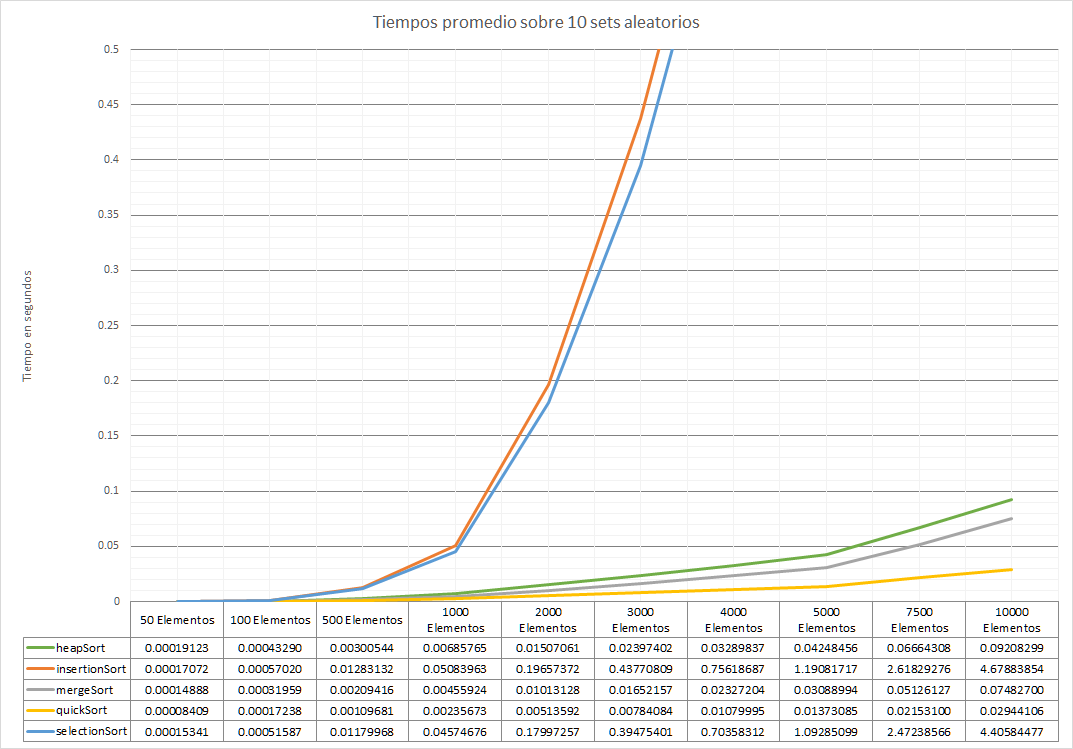
\includegraphics[width=1.2\textwidth]{GraficoCasoRandom}}
  
Es claro que el caso de orden solo afecta descendente en quicksort e insertionsort.
Se ve en la comparación que para pocos elementos el comportamiento de los ordenamientos es similar. Pasando los mil elementos se ve como quicksort e insertsort empeoran notablemente. Para el set mayor, se ve que insertionSort tarda cuatro veces más, y quicksort tarda más de 200 veces lo que tardaba en promedio. El resto de los ordenamientos no se ve afectado notablemente.
En el gráfico es más que notorio como quicksort tomó un orden cuadrático al igual que los ordenamientos por inserción y selección.

En el siguiente gráfico se muestra la comparación explícita del insertion sort:
y a continuación el análogo de quicksort

\makebox[\textwidth][c]{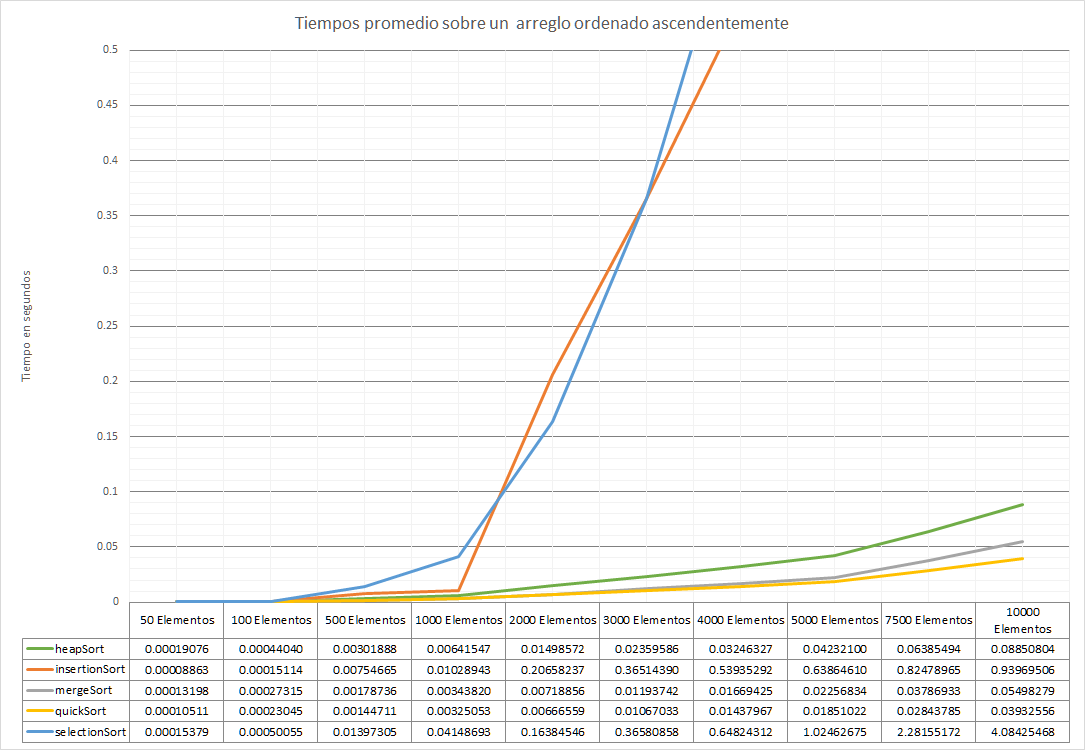
\includegraphics[width=1.2\textwidth]{GraficoCasoAscendente}}
\makebox[\textwidth][c]{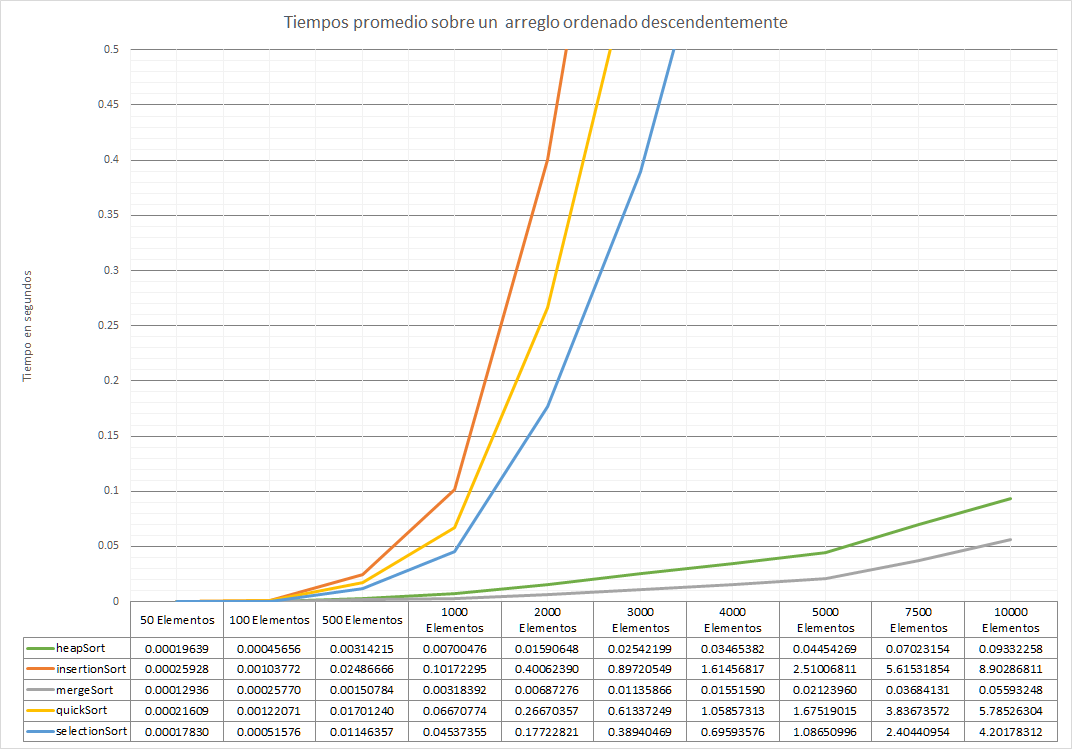
\includegraphics[width=1.2\textwidth]{GraficoCasoDescendente}}
\makebox[\textwidth][c]{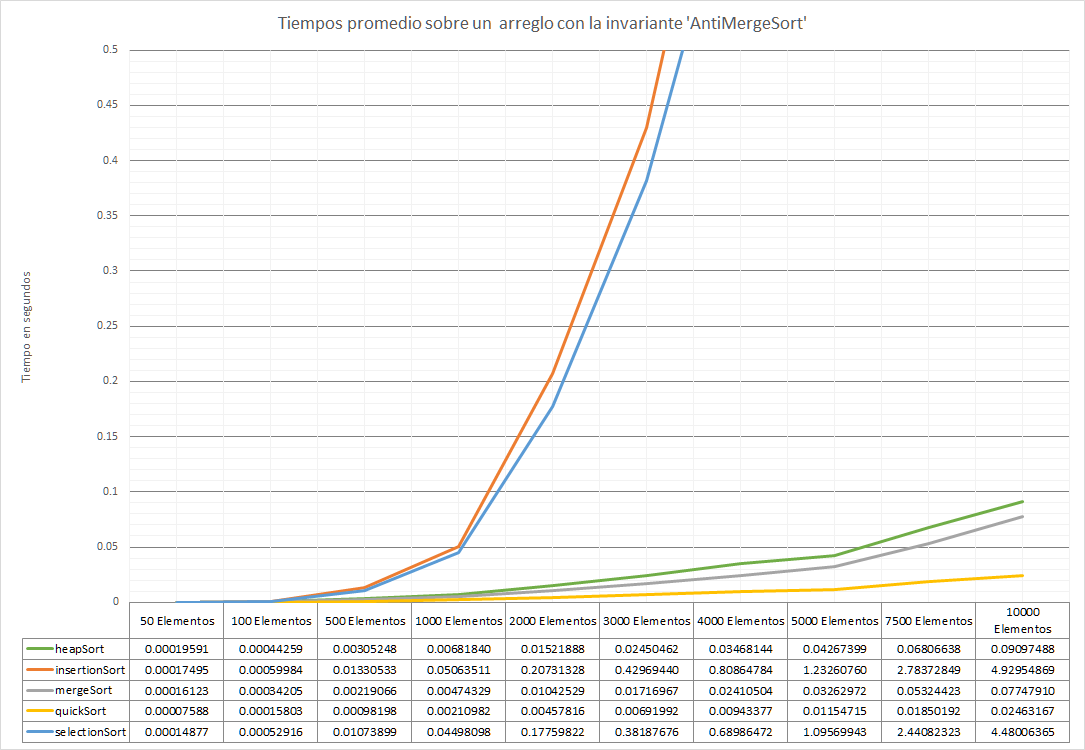
\includegraphics[width=1.2\textwidth]{GraficoCasoAntiMergeSort}}

Las tablas enteras con todas las ejecuciones pueden verse en el anexo al final.


\subsection{Comparación con valores teóricos}

De acuerdo a las complejidades analizadas para el peor caso, se predice que los algoritmos de selección inserción y quicksort tardarán mucho más en ordenar arreglos que heapsort o mergesort. Esto se cumple, con la salvedad que en el análisis teórico para el peor caso se preveía que el ordenamiento por selección tendría peor desempeño que quicksort, lo cual no ocurrió, por ser el set especialmente diseñado para que quicksort se comporte de forma poco eficiente.

Con respecto al caso promedio, los tiempos se cumplieron de forma exactamente coherente con el orden de eficiencia predicho (en orden ascendente) en el análisis teórico: inserción, selección, heapsort, mergesort y quicksort. En síntesis, excepto por el peor caso de quicksort que no fue considerado de forma explícita, el análisis teórico se condice con los valores visualizados en la práctica.


\section{Algoritmo Gale-Shapley}

\subsection{Algoritmo}

El algoritmo de asignación propiamente dicho se reduce a la función homónima:

\begin{minted}[xleftmargin=\parindent,linenos]{python}
codigocodigocodigo
\end{minted}

\subsection{Demostraciones}

\subsubsection{Tiempo polinómico}

Para facilitar la notación de está sección, J será la cantidad de jugadores y E la cantidad de equipos. Para la justificación detallada de cada sentencia del algoritmo, ver los comentarios de la complejidad en el código.

En el algoritmo el primer método que se llama es jugadoresEquiposGS. En caso en que se especifique la creación de los archivos .rtf, el método generarArchivos tiene una complejidad es de orden O(E*J), ya que por cada equipo se debe crear un archivo de longitud igual a la cantidad de jugadores, y lo análogo ocurre a la recíproca.

La carga de archivos con el método cargaDeArchivos naturalmente también de orden O(J*E) ya que por cada jugador que se quiera crear, se debe recorrer un archivo cuya longitud es igual a la cantidad de equipos, y viceversa.

La asignación, donde se genera el matching establece, tiene como condición de corte que no haya más vacantes en los equipos. Considerando esto, el hecho de que a continuación en el algoritmo se itere por cada equipo, y que se verifique para cada uno si todos tiene vacantes, es solo una especificación para lograr cubrir todas las vacantes, por lo que no agregan un orden diferente: simplemente es la forma de implementar que el algoritmo avance a partir de que se cubren distintas vacantes en distintas equipos. Esto implica que cada equipo deberá completar todos sus lugares libres, y como hay igual cantidad de jugadores que de vacantes, el peor caso se considera cuando cada equipo debe preguntarle a todos los jugadores si desean ocupar una vacante: esto es O(J). Como hay E equipos, el orden de la asignación también es O(J*E).

Finalmente, almacenar el archivo de la asignación tiene un orden línea O(J+E). Esto se debe a que por cada equipo, se guarda su número seguido de los números de jugadores que tiene. La cantidad de jugadores que tiene un equipo es igual a sus vacantes (ver demostración en el próximo item de que cada equipo llena todas sus vacantes) y como la cantidad de vacantes totales es igual al número de jugadores, se tiene que se guardó un archivo con J + E números.

El orden cuadrático del algoritmo, entonces, es evidente, ya que es el peor caso de complejidad a lo largo de las funciones del algoritmo. Como O(J*E) es un orden polinomial, el algoritmo es de orden polinomial.

\subsubsection{Matching estable}

Para está demostración, se simplificará la estructura original de la solución implementada. Considerando el primer método llamado "jugadoresEquiposGS", se excluyen las características de la generación de los archivos .'prf', su carga, y el correspondiente almacenamiento del archivo donde se guarda la asignación estable. Entonces, el método se reduce a la asignación propiamente dicha.

Por una cuestión de comodidad, se puede traducir esto a un psuedcódigo basado en la documentación del método de asignación:
'''Mientras haya un equipo con vacantes.'''
    '''El equipo actual ofrece una vacante a su jugador favorito actual'''
        '''Si el jugador esta libre, acepta la vacante'''
              '''Si no esta libre, pero prefiere más al equipo actual, acepta la vacantey el otro equipo pierde a ese jugador.'''

Como hay igual cantidad de jugadores que de vacantes totales, se ve que todos los equipos podrán cubrir todos su puestos. Supongamos que hubiera un equipo "a" que ya ha "ofrecido una vacante" a todos los jugadores de acuerdo con su favoritismo, y ninguno la hubiera aceptado. Esto es decir que todos los jugadores ya han aceptado una vacante en un equipo previamente. Pero esto es una contradicción, porque existe la misma cantidad de jugadores que de vacantes totales, y por hipótesis hay una (al menos) vacante que "a" no puede cubrir. Justamente, la contradicción viene de suponer que un equipo no ha podido satisfacer una de sus vacantes ofreciéndole a todos los jugadores, por lo que esto es falso. Con esto se ve además que la máxima cantidad de "proposiciones" que un equipo puede hacer es igual a la cantidad de vacantes disponibles en total, es decir, con la cantidad de jugadores.

Ahora se demostrar que una vez que cada equipo haya cubierto sus vacantes, no habrá parejas conflictivas (inestabilidades). La misma podría darse entre (j1,a) y (j2,b), donde j1 es un jugador que quiere estar en el equipo b, j2 es un jugador que quiere estar en el equipo a, a es un equipo que prefiere más a j2 sobre j1 y b es un equipo que prefiere más a j1 sobre j2.

Supongamos que a "elige primero". Si j1 aceptó la vacante en a, es porque j1 estaba libre, o bien, porque prefería estar en a que en otro equipo c (no necesariamente c = b).     

Supongamos que era porque estaba solo. Luego b prefiere más a j2 que a j1, porque le ofreció su vacante antes. Si esto no fuera así, b le hubiera ofrecido antes su vacante a j1, y el mismo se hubiera cambiado de equipo, pero esto no sucedió. En este caso se llega a un absurdo, porque por hipótesis b prefiere más a j1 (en otro caso la pareja no es conflictiva y no hay inestabilidad).

Entonces debemos suponer que j1 aceptó la vacante porque estaba en otro equipo c. Luego, se llega al mismo absurdo anterior, porque al fin y al cabo b termina con j2.

Luego, debe ser que b "eligió primero". Si j2 aceptó la vacante en b, es porque j2 estaba libre, o bien, porque prefería estar en b que en otro equipo d (no necesariamente d = b o d = c). En cualquiera de los dos casos se llega a un absurdo similar al anterior.
Todas los caminos a los que conduce la hipótesis "hay una inestabilidad en la asignación final" hacen llegar a una contradicción, por lo que queda probado que la asignación es estable.

No existe posibilidad que quede un equipo con alguna vacante libre, o un jugador sólo, como se probó al principio.

\subsection{Ejecución}
En el anexo junto con el código del algoritmo se ve la posibilidad que brinda de generar los archivos prf. El resultado de una de las ejecuciones fue la siguiente asignación: 

\begin{verbatim}
1: 150 120 119 11 22 175 28 15 78 130
2: 182 200 8 191 44 36 60 134 17 159
3: 189 34 1 138 142 45 190 100 197 187
4: 88 9 132 46 62 91 188 103 145 70
5: 48 20 178 27 168 97 30 176 124 98
6: 125 129 25 86 180 165 106 5 177 12
7: 155 158 31 54 195 93 146 29 24 170
8: 164 63 110 127 109 140 96 160 149 143
9: 154 169 198 161 61 99 84 179 33 151
10: 173 69 35 117 163 65 112 118 104 43
11: 166 76 58 137 185 18 77 94 2 186
12: 51 4 171 199 87 162 19 181 85 80
13: 49 40 55 101 26 123 131 92 114 72
14: 193 115 39 37 135 6 172 38 141 174
15: 10 147 167 73 156 14 133 57 74 152
16: 126 192 136 148 71 23 52 153 111 32
17: 116 196 67 82 64 21 59 68 107 113
18: 105 56 90 66 47 183 7 75 108 16
19: 41 81 102 184 3 122 194 79 157 139
20: 42 83 13 128 53 50 144 89 121 95
\end{verbatim}


\appendix

\section{Ejecución y compilación}

Todo el trabajo fue codificado en Python 3.6.1. 

\subsection{Ordenamientos: Ejecución general}

El programa principal es ejecutado desde el archivo main, especificando por linea de comando el caso a ejecutar, entre "Random" y "Peor", refiriendose a los sets por donde se ejecutaran los ordenamientos. La ejecución consiste de iterar sobre los sets generados previamente y en cada uno ejecutar cada ordenamiento estudiado sobre distintas cantidades del mismo elemento. Este archivo genera un 'SalidaRandom.csv' con las estadisticas necesarias para analizar.

\begin{minted}{shell}
>>> python main.py Random
>>> python main.py Peor
\end{minted}

\subsection{Generación de sets aleatorios}

El script generarSetRandom.py permite generar los sets aleatorios de n numeros (en este caso, n=10000) en un rango determinado. Ejemplo de ejecución:

\begin{minted}{shell}
>>> from generarSetRandom import generarSet
>>> generarSet("set01.txt", 1, 1000000, 10000)
\end{minted}

\subsection{Pruebas de ordenamientos}
Para verificar que los ordenamientos anden correctamente se realizaron varias pruebas unitarias que verfiquen distintos comportamientos desde los casos triviales hasta los casos borde y demás. Todas las pruebas son iguales, e incluyen asserts con ordenamientos aleatorios.

\begin{minted}{shell}
>>> python3 heapTest.py -v
\end{minted}

\subsection{Medición de tiempos}
 Los tiempos de ejecución fueron calculados con el modulo \texttt{time} de Python, en particular su función \texttt{process\_time} \footnote{\url{https://docs.python.org/3/library/time.html\#process\_time}}.

\subsection{Stable matching}
 Para generar un matching estable, se debe importar el archivo matchinGS.py y ejecutar la siguiente línea:
matchingGS(‘ruta de los archivos  de jugadores y su correspondiente nombre sin número’, ‘extensión de los archivos jugadores’, ‘ruta de los archivos de equipos y su correspondiente nombre sin número’, ‘extensión de los archivos de equipos’, ‘nombre completo del archivo donde se guardará la asignación’, cantidad de jugadores, cantidad de equipos, cantidad de vacantes por equipo, ‘y’ si se quieren generar los archivos o cualquier otro caracter en otro caso)

Por ejemplo, para cumplir con la consigna se requieren los siguientes comandos:

\begin{minted}{shell}
>>> from matchingGS import matchingGS
>>> matchingGS('archivos/jugador_', '.prf', 'archivos/equipo_', '.prf', 'asignacion.txt', 200, 20, 10, 'y')
\end{minted}

\section{Tablas de ejecución}

\subsection{Tiempos de ejecución sobre sets aleatorios}

\begin{table}[h]
\centering
\caption{Tiempos de ejecución sobre 10 sets aleatorios}
\resizebox{\textwidth}{!}{\begin{tabular}{lllllllllll}
50 Elementos    & SetRandom01 & SetRandom02 & SetRandom03 & SetRandom04 & SetRandom05 & SetRandom06 & SetRandom07 & SetRandom08 & SetRandom09 & SetRandom10 \\
heapSort        & 0.00019300  & 0.00018855  & 0.00019178  & 0.00020529  & 0.00018293  & 0.00018698  & 0.00019424  & 0.00019802  & 0.00018284  & 0.00018867  \\
insertionSort   & 0.00019945  & 0.00015891  & 0.00012839  & 0.00018014  & 0.00016239  & 0.00016163  & 0.00018052  & 0.00017342  & 0.00016791  & 0.00019444  \\
mergeSort       & 0.00016291  & 0.00014654  & 0.00014624  & 0.00015401  & 0.00014920  & 0.00014525  & 0.00014689  & 0.00014798  & 0.00014500  & 0.00014480  \\
quickSort       & 0.00008861  & 0.00007581  & 0.00008263  & 0.00008232  & 0.00008747  & 0.00008240  & 0.00008242  & 0.00009243  & 0.00008440  & 0.00008239  \\
selectionSort   & 0.00015473  & 0.00015757  & 0.00014861  & 0.00015807  & 0.00015818  & 0.00014677  & 0.00015120  & 0.00015299  & 0.00015108  & 0.00015492  \\
                &             &             &             &             &             &             &             &             &             &             \\
100 Elementos   & SetRandom01 & SetRandom02 & SetRandom03 & SetRandom04 & SetRandom05 & SetRandom06 & SetRandom07 & SetRandom08 & SetRandom09 & SetRandom10 \\
heapSort        & 0.00043570  & 0.00045246  & 0.00044005  & 0.00042592  & 0.00042845  & 0.00043440  & 0.00041988  & 0.00041455  & 0.00044249  & 0.00043516  \\
insertionSort   & 0.00058790  & 0.00064046  & 0.00054841  & 0.00053005  & 0.00067365  & 0.00052636  & 0.00048715  & 0.00049590  & 0.00057678  & 0.00063538  \\
mergeSort       & 0.00034085  & 0.00030815  & 0.00032360  & 0.00032457  & 0.00031131  & 0.00031344  & 0.00031926  & 0.00032349  & 0.00032025  & 0.00031099  \\
quickSort       & 0.00017878  & 0.00016309  & 0.00017036  & 0.00016766  & 0.00015238  & 0.00017618  & 0.00017809  & 0.00019167  & 0.00016401  & 0.00018156  \\
selectionSort   & 0.00053624  & 0.00044922  & 0.00051516  & 0.00052856  & 0.00052489  & 0.00051390  & 0.00051862  & 0.00052146  & 0.00051781  & 0.00053284  \\
                &             &             &             &             &             &             &             &             &             &             \\
500 Elementos   & SetRandom01 & SetRandom02 & SetRandom03 & SetRandom04 & SetRandom05 & SetRandom06 & SetRandom07 & SetRandom08 & SetRandom09 & SetRandom10 \\
heapSort        & 0.00297829  & 0.00302412  & 0.00294132  & 0.00303563  & 0.00305413  & 0.00306853  & 0.00292844  & 0.00296854  & 0.00307565  & 0.00297974  \\
insertionSort   & 0.01235648  & 0.01359664  & 0.01212989  & 0.01256291  & 0.01334884  & 0.01287573  & 0.01298992  & 0.01232904  & 0.01256445  & 0.01355928  \\
mergeSort       & 0.00211735  & 0.00207506  & 0.00200294  & 0.00210409  & 0.00210602  & 0.00207392  & 0.00207665  & 0.00209064  & 0.00224680  & 0.00204810  \\
quickSort       & 0.00105629  & 0.00103137  & 0.00113191  & 0.00104716  & 0.00097052  & 0.00114077  & 0.00130709  & 0.00114264  & 0.00105451  & 0.00108588  \\
selectionSort   & 0.01152360  & 0.01153958  & 0.01241996  & 0.01133049  & 0.01146322  & 0.01228531  & 0.01155788  & 0.01251674  & 0.01120192  & 0.01215812  \\
                &             &             &             &             &             &             &             &             &             &             \\
1000 Elementos  & SetRandom01 & SetRandom02 & SetRandom03 & SetRandom04 & SetRandom05 & SetRandom06 & SetRandom07 & SetRandom08 & SetRandom09 & SetRandom10 \\
heapSort        & 0.00739671  & 0.00694720  & 0.00662311  & 0.00683279  & 0.00688662  & 0.00678391  & 0.00675784  & 0.00681219  & 0.00681572  & 0.00672041  \\
insertionSort   & 0.05100241  & 0.05244503  & 0.04842442  & 0.05063798  & 0.05230036  & 0.05133143  & 0.04899568  & 0.05267124  & 0.05200502  & 0.04858271  \\
mergeSort       & 0.00456525  & 0.00470494  & 0.00455071  & 0.00461912  & 0.00467384  & 0.00457552  & 0.00441806  & 0.00447197  & 0.00453215  & 0.00448089  \\
quickSort       & 0.00234790  & 0.00223786  & 0.00238862  & 0.00225757  & 0.00217189  & 0.00256744  & 0.00237706  & 0.00256044  & 0.00233367  & 0.00232482  \\
selectionSort   & 0.04496951  & 0.04662944  & 0.04389748  & 0.04555453  & 0.04726154  & 0.04648492  & 0.04423733  & 0.04462990  & 0.04494551  & 0.04885741  \\
                &             &             &             &             &             &             &             &             &             &             \\
2000 Elementos  & SetRandom01 & SetRandom02 & SetRandom03 & SetRandom04 & SetRandom05 & SetRandom06 & SetRandom07 & SetRandom08 & SetRandom09 & SetRandom10 \\
heapSort        & 0.01523260  & 0.01514745  & 0.01499430  & 0.01506648  & 0.01513730  & 0.01514470  & 0.01494349  & 0.01490355  & 0.01500769  & 0.01512852  \\
insertionSort   & 0.19201088  & 0.20843868  & 0.19088637  & 0.20495201  & 0.18710003  & 0.19607610  & 0.19952160  & 0.19383391  & 0.19547072  & 0.19744693  \\
mergeSort       & 0.01019977  & 0.01023930  & 0.01023052  & 0.01000460  & 0.00995667  & 0.01017505  & 0.01017236  & 0.01010934  & 0.01008799  & 0.01013720  \\
quickSort       & 0.00521293  & 0.00494697  & 0.00516645  & 0.00492783  & 0.00488734  & 0.00544569  & 0.00523995  & 0.00549807  & 0.00492884  & 0.00510515  \\
selectionSort   & 0.18609935  & 0.18948616  & 0.17618832  & 0.18041831  & 0.18240617  & 0.17892075  & 0.17892672  & 0.17642920  & 0.17546178  & 0.17538898  \\
                &             &             &             &             &             &             &             &             &             &             \\
3000 Elementos  & SetRandom01 & SetRandom02 & SetRandom03 & SetRandom04 & SetRandom05 & SetRandom06 & SetRandom07 & SetRandom08 & SetRandom09 & SetRandom10 \\
heapSort        & 0.02425120  & 0.02387434  & 0.02414011  & 0.02377146  & 0.02410929  & 0.02380476  & 0.02375325  & 0.02389451  & 0.02424637  & 0.02389495  \\
insertionSort   & 0.41653200  & 0.43707999  & 0.46344494  & 0.42481478  & 0.42187480  & 0.43046910  & 0.44544637  & 0.43564340  & 0.43663127  & 0.46514423  \\
mergeSort       & 0.01658727  & 0.01641316  & 0.01661186  & 0.01664745  & 0.01655258  & 0.01660167  & 0.01633104  & 0.01628040  & 0.01666285  & 0.01652746  \\
quickSort       & 0.00768843  & 0.00768781  & 0.00794279  & 0.00745642  & 0.00730129  & 0.00819662  & 0.00793997  & 0.00869121  & 0.00756967  & 0.00793418  \\
selectionSort   & 0.39494834  & 0.39463882  & 0.39689663  & 0.39429853  & 0.39780394  & 0.39295478  & 0.39391488  & 0.39499579  & 0.39344403  & 0.39364438  \\
                &             &             &             &             &             &             &             &             &             &             \\
4000 Elementos  & SetRandom01 & SetRandom02 & SetRandom03 & SetRandom04 & SetRandom05 & SetRandom06 & SetRandom07 & SetRandom08 & SetRandom09 & SetRandom10 \\
heapSort        & 0.03284454  & 0.03317121  & 0.03303558  & 0.03275882  & 0.03270194  & 0.03312007  & 0.03281572  & 0.03249362  & 0.03293303  & 0.03310914  \\
insertionSort   & 0.73809955  & 0.78122650  & 0.76783974  & 0.73013473  & 0.75447225  & 0.76763770  & 0.77887734  & 0.76187592  & 0.71228048  & 0.76942447  \\
mergeSort       & 0.02300822  & 0.02343306  & 0.02342124  & 0.02328943  & 0.02313355  & 0.02297004  & 0.02354313  & 0.02337101  & 0.02330195  & 0.02324881  \\
quickSort       & 0.01065544  & 0.01044370  & 0.01096001  & 0.01008401  & 0.00996224  & 0.01140329  & 0.01128360  & 0.01181481  & 0.01050973  & 0.01088262  \\
selectionSort   & 0.70282919  & 0.69928560  & 0.70064164  & 0.69431765  & 0.70229424  & 0.71497047  & 0.69866235  & 0.69994268  & 0.70156687  & 0.72132049  \\
                &             &             &             &             &             &             &             &             &             &             \\
5000 Elementos  & SetRandom01 & SetRandom02 & SetRandom03 & SetRandom04 & SetRandom05 & SetRandom06 & SetRandom07 & SetRandom08 & SetRandom09 & SetRandom10 \\
heapSort        & 0.04218705  & 0.04252301  & 0.04292750  & 0.04175632  & 0.04291162  & 0.04227332  & 0.04209742  & 0.04247767  & 0.04263719  & 0.04305448  \\
insertionSort   & 1.18204778  & 1.18909509  & 1.23801325  & 1.20648208  & 1.17101943  & 1.19625304  & 1.15185332  & 1.17470414  & 1.16457618  & 1.23412736  \\
mergeSort       & 0.03085920  & 0.03151913  & 0.03105532  & 0.03084717  & 0.03090164  & 0.03082855  & 0.03068934  & 0.03070248  & 0.03090970  & 0.03058693  \\
quickSort       & 0.01348742  & 0.01339856  & 0.01387731  & 0.01308612  & 0.01279298  & 0.01425968  & 0.01398410  & 0.01520034  & 0.01339186  & 0.01383017  \\
selectionSort   & 1.09344189  & 1.09182913  & 1.08739355  & 1.09608341  & 1.09816645  & 1.09037545  & 1.09863278  & 1.08801684  & 1.08548364  & 1.09908680  \\
                &             &             &             &             &             &             &             &             &             &             \\
7500 Elementos  & SetRandom01 & SetRandom02 & SetRandom03 & SetRandom04 & SetRandom05 & SetRandom06 & SetRandom07 & SetRandom08 & SetRandom09 & SetRandom10 \\
heapSort        & 0.06720685  & 0.06698542  & 0.06631842  & 0.06606606  & 0.06628988  & 0.06588071  & 0.06770505  & 0.06685129  & 0.06663839  & 0.06648876  \\
insertionSort   & 2.57472254  & 2.59746984  & 2.65947080  & 2.67775495  & 2.56712238  & 2.59690785  & 2.61323801  & 2.65732562  & 2.64076297  & 2.59815267  \\
mergeSort       & 0.05152882  & 0.05065012  & 0.05108126  & 0.05083490  & 0.05160936  & 0.05160909  & 0.05094111  & 0.05134133  & 0.05152861  & 0.05148814  \\
quickSort       & 0.02149095  & 0.02084428  & 0.02167369  & 0.02034912  & 0.02018938  & 0.02239834  & 0.02201772  & 0.02336442  & 0.02102273  & 0.02195938  \\
selectionSort   & 2.47117228  & 2.46195340  & 2.45594133  & 2.49144226  & 2.55074881  & 2.45745252  & 2.45648722  & 2.46622304  & 2.45988945  & 2.45254629  \\
                &             &             &             &             &             &             &             &             &             &             \\
10000 Elementos & SetRandom01 & SetRandom02 & SetRandom03 & SetRandom04 & SetRandom05 & SetRandom06 & SetRandom07 & SetRandom08 & SetRandom09 & SetRandom10 \\
heapSort        & 0.09234720  & 0.09180443  & 0.09170632  & 0.09235643  & 0.09237836  & 0.09184556  & 0.09126658  & 0.09187549  & 0.09198058  & 0.09326896  \\
insertionSort   & 4.72838785  & 4.82092053  & 4.71846541  & 4.64045077  & 4.54181549  & 4.66178385  & 4.71195490  & 4.69176563  & 4.71393896  & 4.55890200  \\
mergeSort       & 0.07408563  & 0.07491511  & 0.07442679  & 0.07556444  & 0.07424022  & 0.07440036  & 0.07488256  & 0.07554801  & 0.07454557  & 0.07566138  \\
quickSort       & 0.02859854  & 0.02852403  & 0.02988460  & 0.02795936  & 0.02736539  & 0.03078863  & 0.03012384  & 0.03184481  & 0.02881059  & 0.03051086  \\
selectionSort   & 4.39602486  & 4.53192356  & 4.42551569  & 4.38844704  & 4.39688216  & 4.38836099  & 4.37352012  & 4.36608303  & 4.38014397  & 4.41154632 
\end{tabular}}
\end{table}

\subsection{Tiempos de ejecución sobre sets de peores casos}

\begin{table}[h]
\centering
\caption{Tiempos de ejecución sobre sets de peores casos}
\begin{adjustbox}{width=\textwidth,totalheight=\textheight,keepaspectratio}
\tiny
\begin{tabular}{lllllllllll}
50 Elementos    & SetPeorCasoAscendente & SetPeorCasoDescendente & SetPeorCasoMergesort \\
heapSort        & 0.00019076            & 0.00019639             & 0.00019591           \\
insertionSort   & 0.00008863            & 0.00025928             & 0.00017495           \\
mergeSort       & 0.00013198            & 0.00012936             & 0.00016123           \\
quickSort       & 0.00010511            & 0.00021609             & 0.00007588           \\
selectionSort   & 0.00015379            & 0.00017830             & 0.00014877           \\
                &                       &                        &                      \\
100 Elementos   & SetPeorCasoAscendente & SetPeorCasoDescendente & SetPeorCasoMergesort \\
heapSort        & 0.00044040            & 0.00045656             & 0.00044259           \\
insertionSort   & 0.00015114            & 0.00103772             & 0.00059984           \\
mergeSort       & 0.00027315            & 0.00025770             & 0.00034205           \\
quickSort       & 0.00023045            & 0.00122071             & 0.00015803           \\
selectionSort   & 0.00050055            & 0.00051576             & 0.00052916           \\
                &                       &                        &                      \\
500 Elementos   & SetPeorCasoAscendente & SetPeorCasoDescendente & SetPeorCasoMergesort \\
heapSort        & 0.00301888            & 0.00314215             & 0.00305248           \\
insertionSort   & 0.00754665            & 0.02486666             & 0.01330533           \\
mergeSort       & 0.00178736            & 0.00150784             & 0.00219066           \\
quickSort       & 0.00144711            & 0.01701240             & 0.00098198           \\
selectionSort   & 0.01397305            & 0.01146357             & 0.01073899           \\
                &                       &                        &                      \\
1000 Elementos  & SetPeorCasoAscendente & SetPeorCasoDescendente & SetPeorCasoMergesort \\
heapSort        & 0.00641547            & 0.00700476             & 0.00681840           \\
insertionSort   & 0.01028943            & 0.10172295             & 0.05063511           \\
mergeSort       & 0.00343820            & 0.00318392             & 0.00474329           \\
quickSort       & 0.00325053            & 0.06670774             & 0.00210982           \\
selectionSort   & 0.04148693            & 0.04537355             & 0.04498098           \\
                &                       &                        &                      \\
2000 Elementos  & SetPeorCasoAscendente & SetPeorCasoDescendente & SetPeorCasoMergesort \\
heapSort        & 0.01498572            & 0.01590648             & 0.01521888           \\
insertionSort   & 0.20658237            & 0.40062390             & 0.20731328           \\
mergeSort       & 0.00718856            & 0.00687276             & 0.01042529           \\
quickSort       & 0.00666559            & 0.26670357             & 0.00457816           \\
selectionSort   & 0.16384546            & 0.17722821             & 0.17759822           \\
                &                       &                        &                      \\
3000 Elementos  & SetPeorCasoAscendente & SetPeorCasoDescendente & SetPeorCasoMergesort \\
heapSort        & 0.02359586            & 0.02542199             & 0.02450462           \\
insertionSort   & 0.36514390            & 0.89720549             & 0.42969440           \\
mergeSort       & 0.01193742            & 0.01135866             & 0.01716967           \\
quickSort       & 0.01067033            & 0.61337249             & 0.00691992           \\
selectionSort   & 0.36580858            & 0.38940469             & 0.38187676           \\
                &                       &                        &                      \\
4000 Elementos  & SetPeorCasoAscendente & SetPeorCasoDescendente & SetPeorCasoMergesort \\
heapSort        & 0.03246327            & 0.03465382             & 0.03468144           \\
insertionSort   & 0.53935292            & 1.61456817             & 0.80864784           \\
mergeSort       & 0.01669425            & 0.01551590             & 0.02410504           \\
quickSort       & 0.01437967            & 1.05857313             & 0.00943377           \\
selectionSort   & 0.64824312            & 0.69593576             & 0.68986472           \\
                &                       &                        &                      \\
5000 Elementos  & SetPeorCasoAscendente & SetPeorCasoDescendente & SetPeorCasoMergesort \\
heapSort        & 0.04232100            & 0.04454269             & 0.04267399           \\
insertionSort   & 0.63864610            & 2.51006811             & 1.23260760           \\
mergeSort       & 0.02256834            & 0.02123960             & 0.03262972           \\
quickSort       & 0.01851022            & 1.67519015             & 0.01154715           \\
selectionSort   & 1.02462675            & 1.08650996             & 1.09569943           \\
                &                       &                        &                      \\
7500 Elementos  & SetPeorCasoAscendente & SetPeorCasoDescendente & SetPeorCasoMergesort \\
heapSort        & 0.06385494            & 0.07023154             & 0.06806638           \\
insertionSort   & 0.82478965            & 5.61531854             & 2.78372849           \\
mergeSort       & 0.03786933            & 0.03684131             & 0.05324423           \\
quickSort       & 0.02843785            & 3.83673572             & 0.01850192           \\
selectionSort   & 2.28155172            & 2.40440954             & 2.44082323           \\
                &                       &                        &                      \\
10000 Elementos & SetPeorCasoAscendente & SetPeorCasoDescendente & SetPeorCasoMergesort \\
heapSort        & 0.08850804            & 0.09332258             & 0.09097488           \\
insertionSort   & 0.93969506            & 8.90286811             & 4.92954869           \\
mergeSort       & 0.05498279            & 0.05593248             & 0.07747910           \\
quickSort       & 0.03932556            & 5.78526304             & 0.02463167           \\
selectionSort   & 4.08425468            & 4.20178312             & 4.48006365           
\end{tabular}
\end{adjustbox}
\end{table}

\end{document}
